%windowsでTeXWorksでコンパイルするときはpLaTeX(ptex2pdf)を指定
\documentclass[11pt]{report}
%ここで文章の仕様を決定。Chapterを章とかの日本語にしたいならjreport。
\usepackage[dvipdfmx]{graphicx}%画像の読み込みに必要
\usepackage[top=20truemm, bottom=20truemm, left=20truemm, right=20truemm]{geometry}%余白設定
\usepackage{here}%画像の自動位置調整を禁止するパッケージ。これがないと勝手に画像が移動して不便

\usepackage{amsmath}%一部の数学記号に必要なパッケージ。
\usepackage{physics}%物理で必要な記述に便利なパッケージ。おすすめ
\usepackage{comment}%複数行コメントに使うパッケージ
%\usepackage{indentfirst}
%これはsectionの最初でも文頭にスペースを入れるためのパッケージ。必要ならコメントアウトをはずして

%あとこのTeXデータはそのままテンプレートとして使用してもOK
%導入したパッケージのおかげで情報科学概論で与えられるテンプレートよりも使いやすいと思う
\title{LaTeXてんぷら}
\author{Sugoi Tempra}

\begin{document}
\maketitle%タイトル作成。上で書いた\titleや\authorが出力される
\tableofcontents%目次作成。これだけで自動で全部やってくれるよ

\chapter{TeXの導入方法}
\section{Windows}
以下は世界的にもスタンダードなディストリビューションであるTeXLive2016のインストール方法。\\
https://www.tug.org/texlive/acquire-netinstall.htmlからinstall-tl-windows.exeをダウンロードし、実行。(2GBくらいはディスクに空きが必要だったと思う。あと結構時間かかる)デフォルトならCドライブの直下に置かれるはず。

インストールが終われば、TeXの基本型組と各種パッケージに加えて、TeXWorksというそれなりに使いやすいエディタもついてくる。適当にショートカットでも作っておこう。あとコンパイル時はpLaTeX(ptex2pdf)を指定すること。

Windowsでどうしてもターミナルで作業したいっていう人はCygwinなりChocolatey+Powershellなりを入れるとよい。\\
あとはwindows10なら開発者モードでUbuntu for Windowsが使えるのでそれを導入してみるとか

\section{Mac}
\subsection{直接インストーラをダウンロード}
https://www.tug.org/mactex/からMacTeX.pkgをダウンロードし、適当なディレクトリにおいて実行。あとはそのまま指示に従えばよい。このMacTeXはTeXLive2016をベースに作られている。\\
そのまま実行すればエディタとしてTeXShopがインストールされる。これならシェルを使わずコンパイルからpdf出力まで行えるので、適当にショートカットでも作っておこう。
\subsection{全部シェルでやりたい人}
まずapt-getのパッケージをアップデートしておく
\begin{center}
sudo apt-get update
\end{center}
TeXパッケージのインストールは
\begin{center}
sudo apt-get install mactex
\end{center}
を実行。(念のため古いTeXが入っているときはそれをrmしておくといいかも)コンパイルは、作業中のディレクトリにsample.texがあるとしたら
\begin{center}
platex sample.tex\\
dvipdfmx sample.dvi\\
open sample.pdf
\end{center}
これでpdfで出力されるはず。\\
エディタはvimとか...まあ、好きなやつをapt-getしよう。
\chapter{TeXの基本}
以下では簡単な数式の入力例を示します。\\
なお、文字列で数式を入力したい場合は$A^2+B^2=C^2$こんなかんじ。
\section{数式基本}
\begin{equation}
\frac{\pi^2}{6}=\sum_{n=1}^{\infty}\frac{1}{n^2}
\end{equation}
%\frac{A}{B}で分数A/Bが出力される。また特殊記号(円周率とか和とか)は適宜コマンドが用意されている(大抵\英単語)
%下付き添え字は_上つき添え字は^で表す
改行を含む数式の場合
\begin{eqnarray}
f(x)&\equiv&ABC\\
&=&DE\\
&=&F
\end{eqnarray}
%こんなかんじ。改行は\\で行い、&&で挟んだところを揃えてくれる
\section{physicsパッケージの機能}
以下はphysicsパッケージ独自の機能(デフォルトで同様の記述ができるものもあるが、このパッケージを使ったほうが楽に書ける)\\
bra-ket記法
%physicsパッケージの詳細なコマンドは添付のphysics.pdf参照。
\begin{equation}
\hat{H}\ket{\Psi}=-i\hbar\dv{t}\ket{\Psi}
\end{equation}
%この文中の\ketや\dvはphysicsパッケージ独自の機能。
括弧の自動調整
\begin{eqnarray}
(\frac{A}{B}+\int_0^\infty f(x) \dd x)=C\\
\qty(\frac{A}{B}+\int_0^\infty f(x) \dd x)=C
\end{eqnarray}
%\qtyを最初の左括弧の前に入れることで括弧の大きさを自動で調整してくれる
%\left(ABC\right)みたいにしてもできるけど、こっちのが楽
いろいろ演算子とか
\begin{eqnarray}
\vb{A}\vdot\vb{B}=C\\
\vb{A}\cross\vb{B}=C\\
\grad{F(x)}=\vb{A}(x)\\
\div{\vb{A}}(x)=C(x)\\
\curl{\vb{A}}(x)=C(x)\\
\var(E-TS)
\end{eqnarray}
行列も楽に書けるよ
\begin{equation}
\mqty(a & b \\ c & d)
\end{equation}

%これ以外もいろいろあるけど適宜pdfみて
\chapter{応用編}
\section{画像の貼り付け}
\subsection{TeXLive2015以降}
昔のTeXだと使える形式がepsだけだったり画像のピクセル数を指定しなくちゃいけなくて面倒だったが、TeXLive2015以降でgraphicxパッケージが更新されたことでだいぶ使いやすくなった。\\
あらかじめTeXデータと同じフォルダに画像データを置いておくこと。\\
(注:大学のPCはTeXLive2013なのでこのセクションの方法ではエラーを吐くので、以下のコードはコメントアウトしてある)

\begin{comment}
%この\begin{comment}~\end{comment}までコメントアウトされている。色変えしてくれないけど
\begin{center}
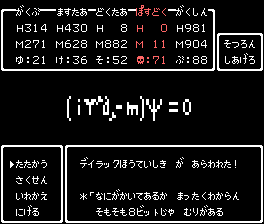
\includegraphics[width=5cm]{texsenden.png}
\end{center}
%\begin{center},\end{center}がないと左寄せになる
%大きさの部分を指定せずに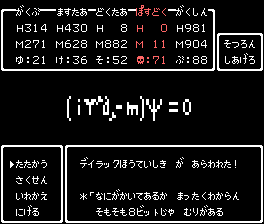
\includegraphics{texsenden.png}とするとそのままの大きさで出力される
また画像にキャプションをつけたい場合はfigure環境を使う:
\begin{figure}
\begin{center}
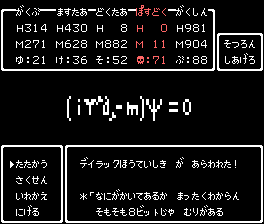
\includegraphics[width=5cm]{texsenden.png}
\end{center}
\caption{8bitいいよね}
\end{figure}

\end{comment}

\subsection{TeXLive2015以前}
大学のPCはTeXLive2013をベースとしたMacTeXをディストリビューションとしている。今更新をするよう頼んではいるが、現在(2016/12/03)ではまだ更新されていない。そのため古い画像の貼り付け方もここで説明しておく。

\subsubsection{eps形式の画像}
もともとTeXではeps形式が推奨環境であったため、古いTeXディストリビューションではこれを使うほうが簡単に貼り付けられる。しかしepsはほかのフォーマットに比べて非常に重い(数十倍になる)うえ、近年ではそこまで一般的な形式ではないので、最新の環境ではこれを使うことは(互換性を気にしているのでない限り)お勧めしない。

なおjpg,pngなどほかのフォーマットからepsにする方法は、Macならデフォルトで入っているImageMagickのconvertコマンドを使うと楽。\\
いまのディレクトリにtest.pngが置かれているとして
\begin{center}
convert test.png test.eps
\end{center}
で変換できる。\\
けどまあ別に適当なツールかWeb上の変換サービスを使ってもいいよ

\begin{figure}
\begin{center}
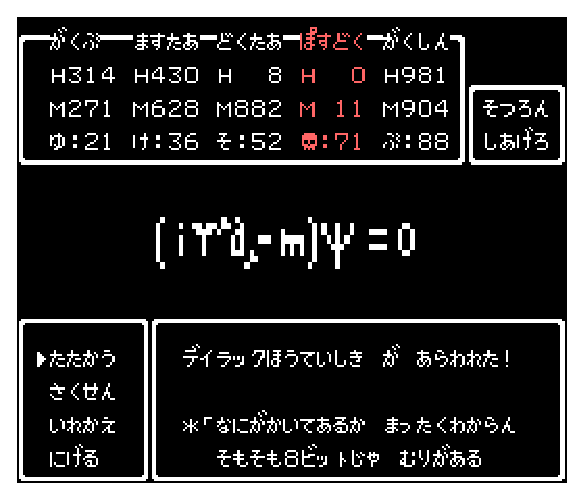
\includegraphics[width=5cm]{texsenden.eps}
\caption{8bitいいよね}
\end{center}
\end{figure}

\subsubsection{jpg, pngなど}
貼る画像のピクセル数をbbで指定する必要がある。
例えばtexsenden.pngは幅264,高さ224ピクセルなので
\begin{center}
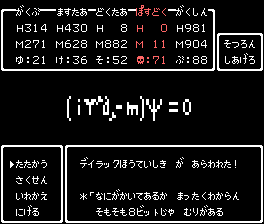
\includegraphics[width=5cm, bb=0 0 264 224]{texsenden.png}
\end{center}
これで貼り付けられる。


\section{ラベルと参照}
文中で式や画像を引用したいときにはラベルを設定するとよい。
\begin{equation}
(i\gamma^\mu\partial_\mu-m)\psi=0
\label{Dirac}%これがラベル。\begin~\endの部分がラベルの対象になる
\end{equation}
(\ref{Dirac})はDirac eq.である。\\
式番号を自動で参照してくれる。ただし新たにラベルを付けたときはコンパイルを2回行うこと(TeXの仕様)
\section{式番号の削除}
TeXはequation環境で書いた数式に標準で式番号をつけてくれるが、これを消したい場合は
\begin{equation}
ABC=Z\nonumber
\end{equation}
でできる。特にeqnarrayで最終行だけ式番号をつけたいとき
\begin{eqnarray}
f(x)&=&(x+a)^2+bx \nonumber \\
&=&x^2+2ax+a^2+bx\nonumber \\
&=&x^2+(2a+b)x+a^2
\end{eqnarray}
こんな感じ。


\section{表の作成}
table環境で行う。(Excelで作って貼ってもいいけど)個人的にはちょっとわかりにくい気がする。
数学の行列はphysicsパッケージのmqtyを使って書いたほうが楽
\begin{table}
  \begin{tabular}{|c|c|c|c|c|} \hline
    がくぶ & ますたあ & どくたあ &ぽすどく & がくしん \\ \hline \hline
    H314 & H430      & H\ \ \ 8         & H\ \ \ 0        &H981 \\
    M271 & M628    & M882   & M\ 11     &M904 \\ 
    ゆ:21 & け:36     & そ:71    &しに        &ぶ:88  \\ \hline
  \end{tabular}
\end{table}


\section{引用の記述}
参考文献とかはこんな感じでいける\\
このてんぷらはM.Tempra\cite{Tempra}を参考にした。\\
この式の証明はS.Superman\cite{Awesome}参照。
\begin{thebibliography}{10}%ここの数字は引用数の上限。適当に大きい数字を入れておくだけでもいい
  \bibitem{Tempra}M.Tempra, ``すごい天ぷらの作り方'', おさしみ書店(2016)%本の引用例
  \bibitem{Awesome}S.Superman, ``Awesome Osashimi'', Fabulous.Phys. 133-138(2016)%論文の引用例
\end{thebibliography}
\end{document}